% ##################################################################################################################
\chapter{Sochi}
\label{ch:sochi}
\hfill \textbf{Author:} Marcel Rieser

\editdone{This text has undergone the professional edit. Please no grammatical changes anymore! They are most-probably wrong.}

% ##################################################################################################################
Major sport events usually attract huge crowds of spectators, as well as media
reporters, necessitating numerous official helpers in various locations to guide and
support attendants; naturally, all athletes must also be at
the right place at the right time. For large, international contests like
Olympic games or soccer championships, accommodations are rarely close to the
event facilities, making it necessary to transport spectators, media, helpers
and athletes efficiently over long distances. As such events typically run for
multiple days, or even weeks, with ever-changing combinations of locations and
times where actual competitions take place, substantial planning is required to
ensure that all attendants and participants reach their event locations in time.

Masterconcept Consulting \gls{gmbh}, an Austrian consulting company, has positioned
itself to provide high-level concepts for large sport events. To better serve its clients, 
it developed \gls{itsos}, a \gls{gis}-based system to support its transport
planners in the creation of mobility concepts for major events, as well as 
regional planning. When simulating the planned
events, \gls{itsos} depends heavily on \gls{matsim} to verify that special infrastructure
at major events can handle transport within required time frames, to and from
specific event locations.

\gls{senozon} was responsible for integrating \gls{matsim} with \gls{itsos} and adding \gls{itsos}-specific
functionality to \gls{matsim}. Together, they created a test scenario depicting the
2014 Olympic winter games in Sochi.

% ========================================================================================
\section{System Overview}
\gls{itsos} used \gls{arcgis} for storing and editing infrastructure data, like road
and train networks and event facilities. A custom plug-in also provided a
graphical user interface inside \gls{arcgis} to specify transit routes and schedules,
vehicle types and their assignments to lines and departures, as well as methods
describing expected travel demand. Transport planners could create and manage
scenarios and scenario variants directly from the custom user interface
available inside \gls{arcgis}.

After successful modeling of a scenario in \gls{arcgis}, a planner could export
the network and transit schedule in \gls{matsim}'s \gls{xml} format directly from \gls{itsos} to a
local directory. The travel demand information, consisting of activity-chains,
with zone- or facility-references and number of persons having such a
chain, was exported as tabular information. A special program created a \gls{matsim}
population file from this tabular data, along with a default \gls{configfile}.

The user could then start the \gls{matsim} simulation, using a simple bat-file
on Windows. After the simulation ended,  events were preprocessed and
imported into a database, from which they could be queried and used within \gls{arcgis}
for analysis and visualization purposes.

% ========================================================================================
\section{Extensions to MATSim}
The various groups at major sport events require different handling;
in addition to athletes, there are media reporters, officials,
helpers, caterers, and, of course, many spectators. Persons from different
groups attending the same event will have different requirements about when
to be at the event location, what entrance to use for the event
location and the kind of transport necessary to reach the location. For this reason,
supporting sub-populations for \gls{replanning} and scoring was an important issue.
Different transit offerings were also defined for different agent groups,
because spectator mass transport must usually be separate from
athlete and official transport.

To facilitate transport planners' work, transit lines in
\gls{itsos} were defined with adaptive schedules; given a base headway,
additional departures were scheduled between iterations, if high
occupancy was expected to occur on a line during specific hours. This adjustment was based
on a rule set that ensured a minimum duration for the shorter headway, as well
as a minimum duration for the base headway between the shorter headways.
Figure~\ref{fig:sochi:adaptiveSchedule} shows the graphical schedule of an
adaptive transit line after 80\,iterations.

\createfigure%
{Bus schedule with automatically adapted headways}%
{Bus schedule with automatically adapted headways based on simulated demand for
bus line from Sochi (Central Bus Hub) to Krasnaya Polyana (Hub)}%
{\label{fig:sochi:adaptiveSchedule}}%
{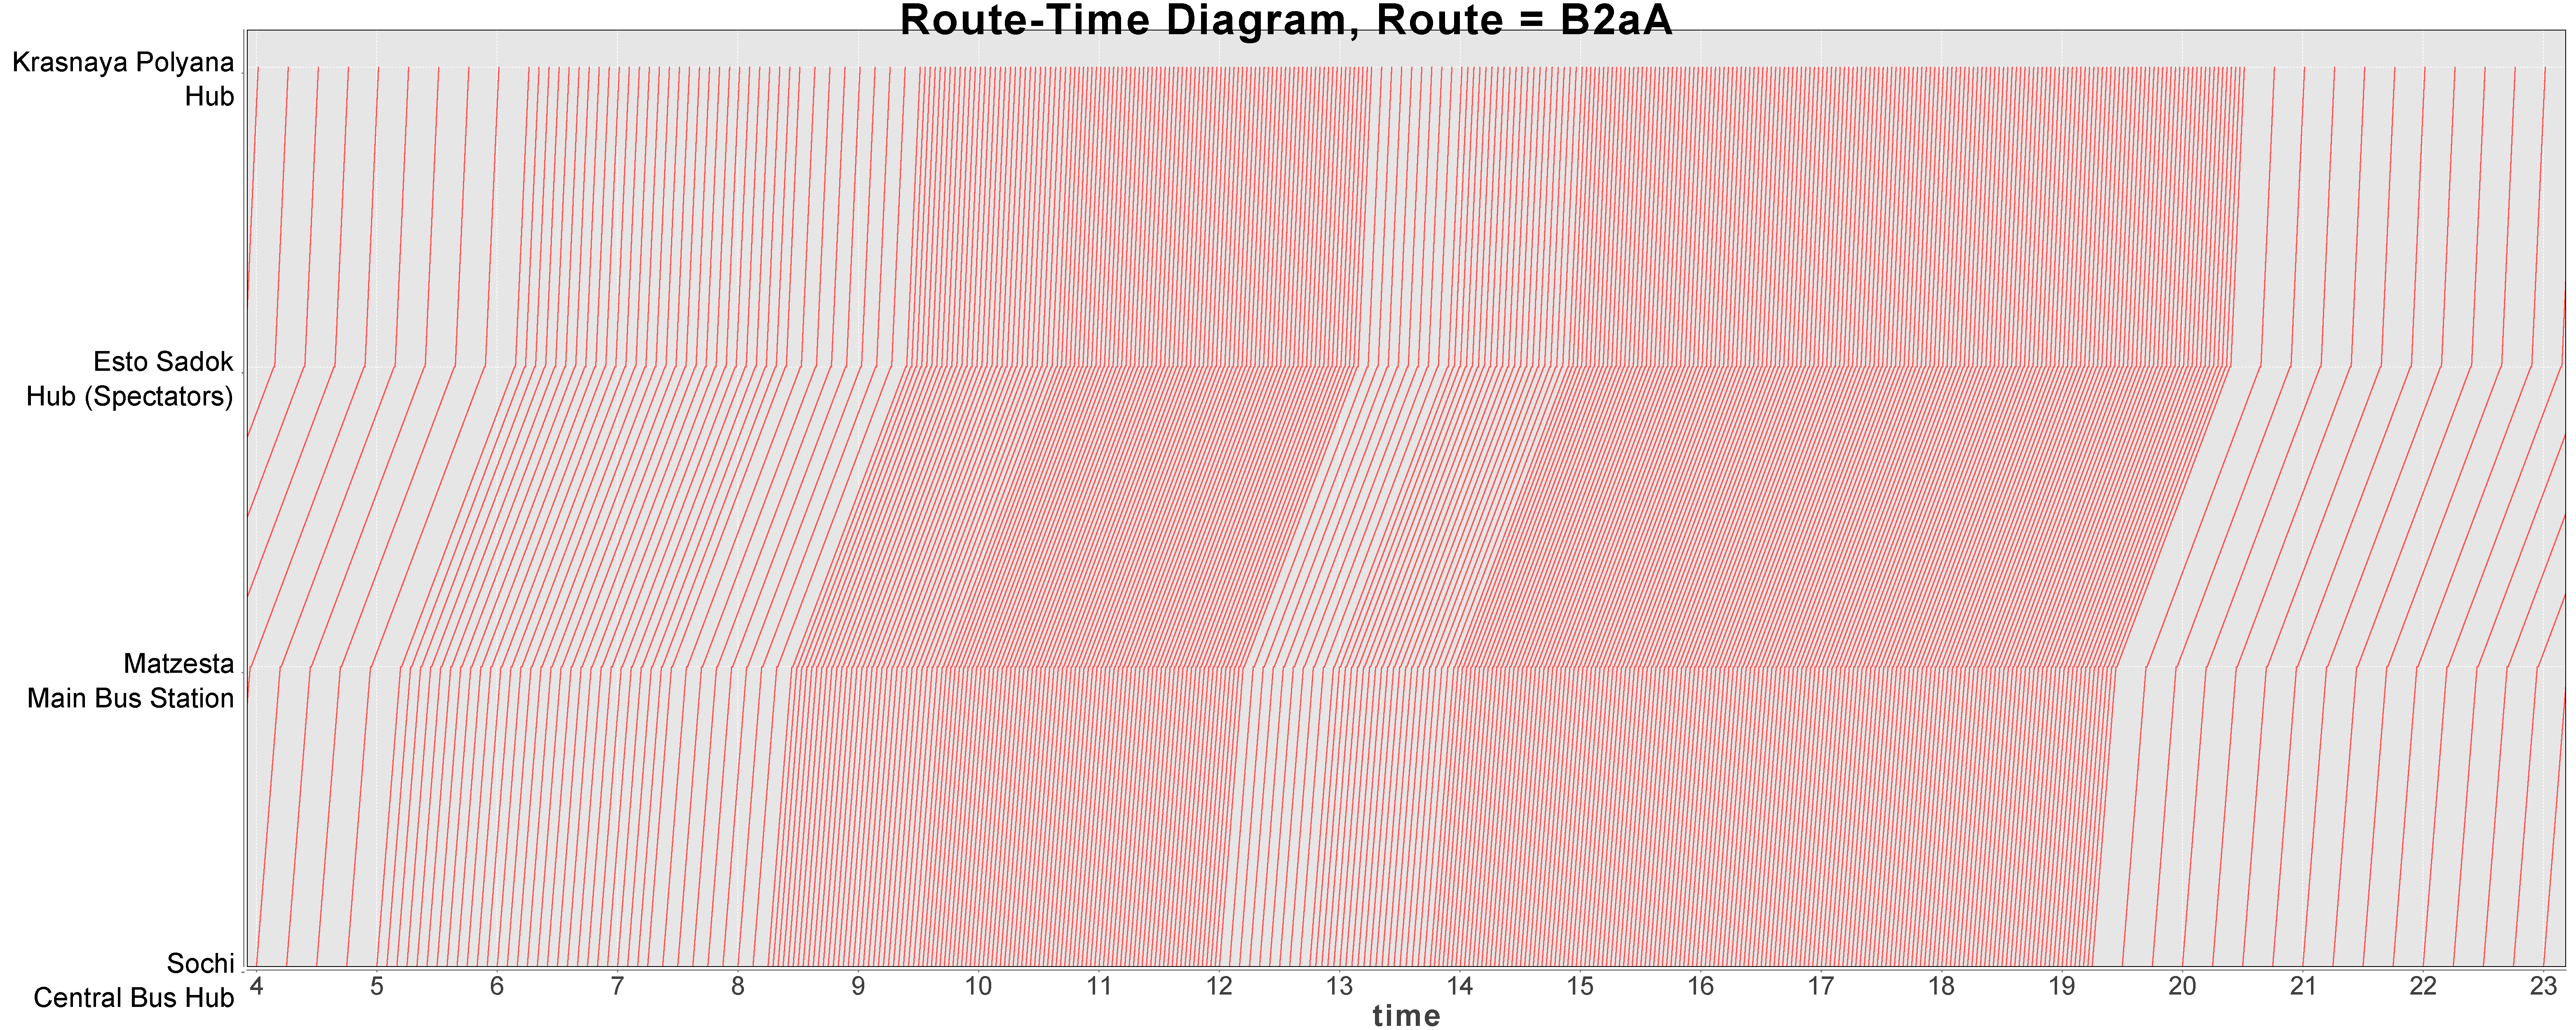
\includegraphics[width=1.\textwidth,angle=0]{./scenarios/figures/sochi_adaptiveSchedule.pdf}}%
{}

In addition to private car traffic and schedule-based public transport, 
athletes, media and officials also use special transportation offerings:
shuttle buses, or even limousine services operating on demand, between only two
or more fixed locations. Termed ``transit on demand'' in \gls{itsos}, transit lines
with stops along a route were defined, but without scheduled departures. 
Instead, a within-day-like operator was implemented, scheduling vehicles
whenever someone from an agent group wished to depart. The
rule-based operator had additional constraints, like minimum occupancy of
on-demand vehicles before departure (to prevent every on-demand vehicle
transporting only a single agent), as well as a maximum waiting time before
departure for such vehicles (to prevent agents in remote locations having to
wait forever).

At sport events, large number of spectators have to share both common entrances
to event facilities and common access paths to those facilities. This
made it necessary to simulate more detailed pedestrian flows (in certain places) 
than just the default \gls{teleportation} approach typically used by
\gls{matsim}. For Olympic games, this was even more crucial because,
in several locations, security checks created additional
bottlenecks. This requirement was solved by implementing a special router for
the walk mode, along with a custom departure handler. The router tried to find a
path on the network for walk legs, assessing distance from the closest walk
link to/from a facility to decide if the link functions as an access to the
facility or not. If no nearby link was found, or no route found between
two access links, an empty route was stored in the leg. The departure handler
checked whether the route was empty or not, either teleporting the agent or putting it
on a walk link in the network. Walk links are regular queue-based network links
with capacity and free-speed set, according to the simplified physics of
directed pedestrian flows. This approach readily allowed modeling of security
screening gates' bottleneck effects and considered essential
walk path locations where necessary. These were modeled, omitting them
on non-critical routes. Figure~\ref{fig:sochi:pedestrians}
shows an example of simulated pedestrian movements at Krasnaya Polyana, the
mountain area near Sochi where numerous events took place.  
%
\createfigure%
{Simulated pedestrians at Krasnaya Polyana hub}%
{Simulated pedestrians (red circles) at Krasnaya Polyana hub. Transit vehicles
(incl. cable cars) shown as green boxes, transit stops as blue circles}%
{\label{fig:sochi:pedestrians}}%
{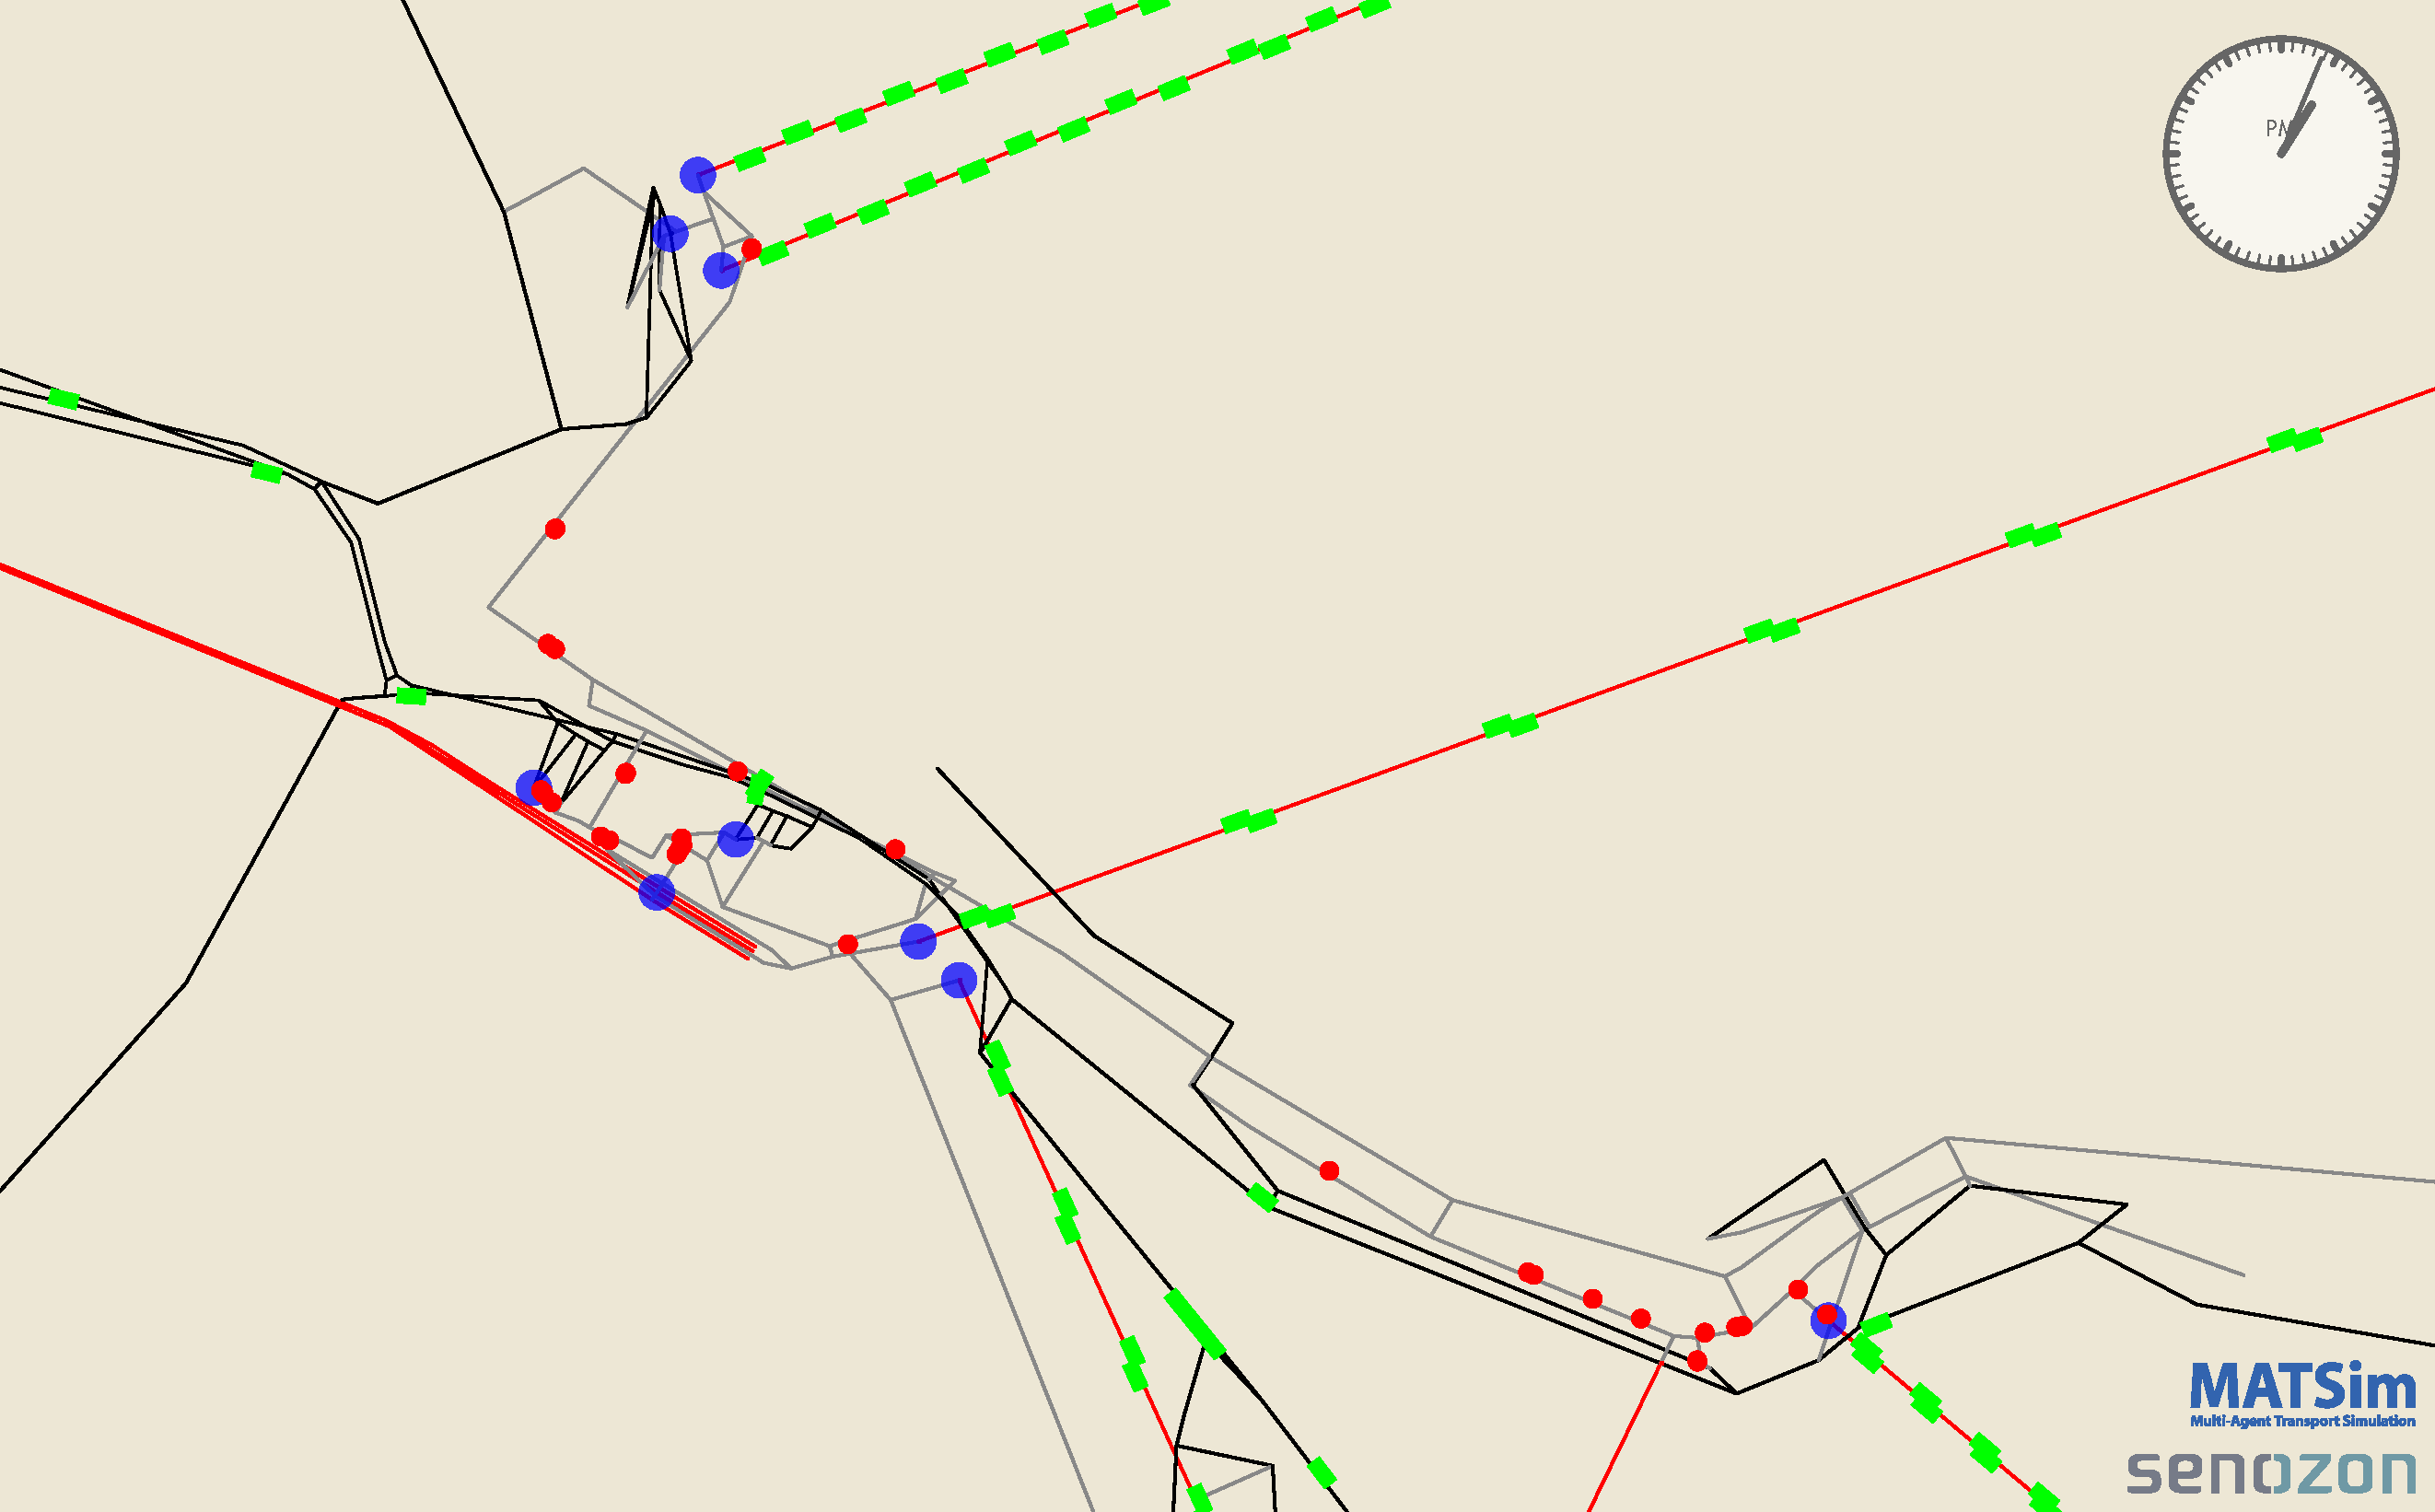
\includegraphics[width=1.\textwidth,angle=0]{./scenarios/figures/sochi_pedestrians.pdf}}%
{}
%

% ========================================================================================
\section{Simulation of Sochi}
To test \gls{itsos} applicability for major events transportation planning,
a model of the 2014 Olympic winter games in Sochi (Russia) was built. Data was
either collected either by Masterconcept employees or cooperating companies, or
received from Russian governmental institutions.

Road and train networks were modeled in \gls{arcgis}, using the \gls{itsos} extensions.
The transit schedule included 55\,transit lines, a mix of bus lines, train lines,
and cable cars, going up into the mountain areas. 24 of those lines were
defined to be adaptive, 19\,lines operated on-demand as shuttle services.

Travel demand was defined for each day of the games, based on the actual schedules,
making assumptions about how many spectators would visit each different
competition during the day. While size of event facilities can be used as a
upper limit for number of spectators, substantial experience and knowledge from
Masterconcept was used to define actual numbers of people expected at each
event.

Events often start and end at different times of day, because many event locations share, at least partially, a
common route to reach them; it was important to simulate whether the transport services offered could
cope with the combined travel demand generated by multiple, separate events.

A typical simulation run of Sochi included about 150\,000\,agents. To speed up simulations, parallel events handling and parallel qsim was used. The simulation generated around 15\,million events per iteration.
%
Figure~\ref{fig:sochi:model} shows a screenshot of the Sochi scenario, visualized in Via.
%
\createfigure%
{Overview of the Sochi model}%
{Overview of the Sochi model}%
{\label{fig:sochi:model}}%
{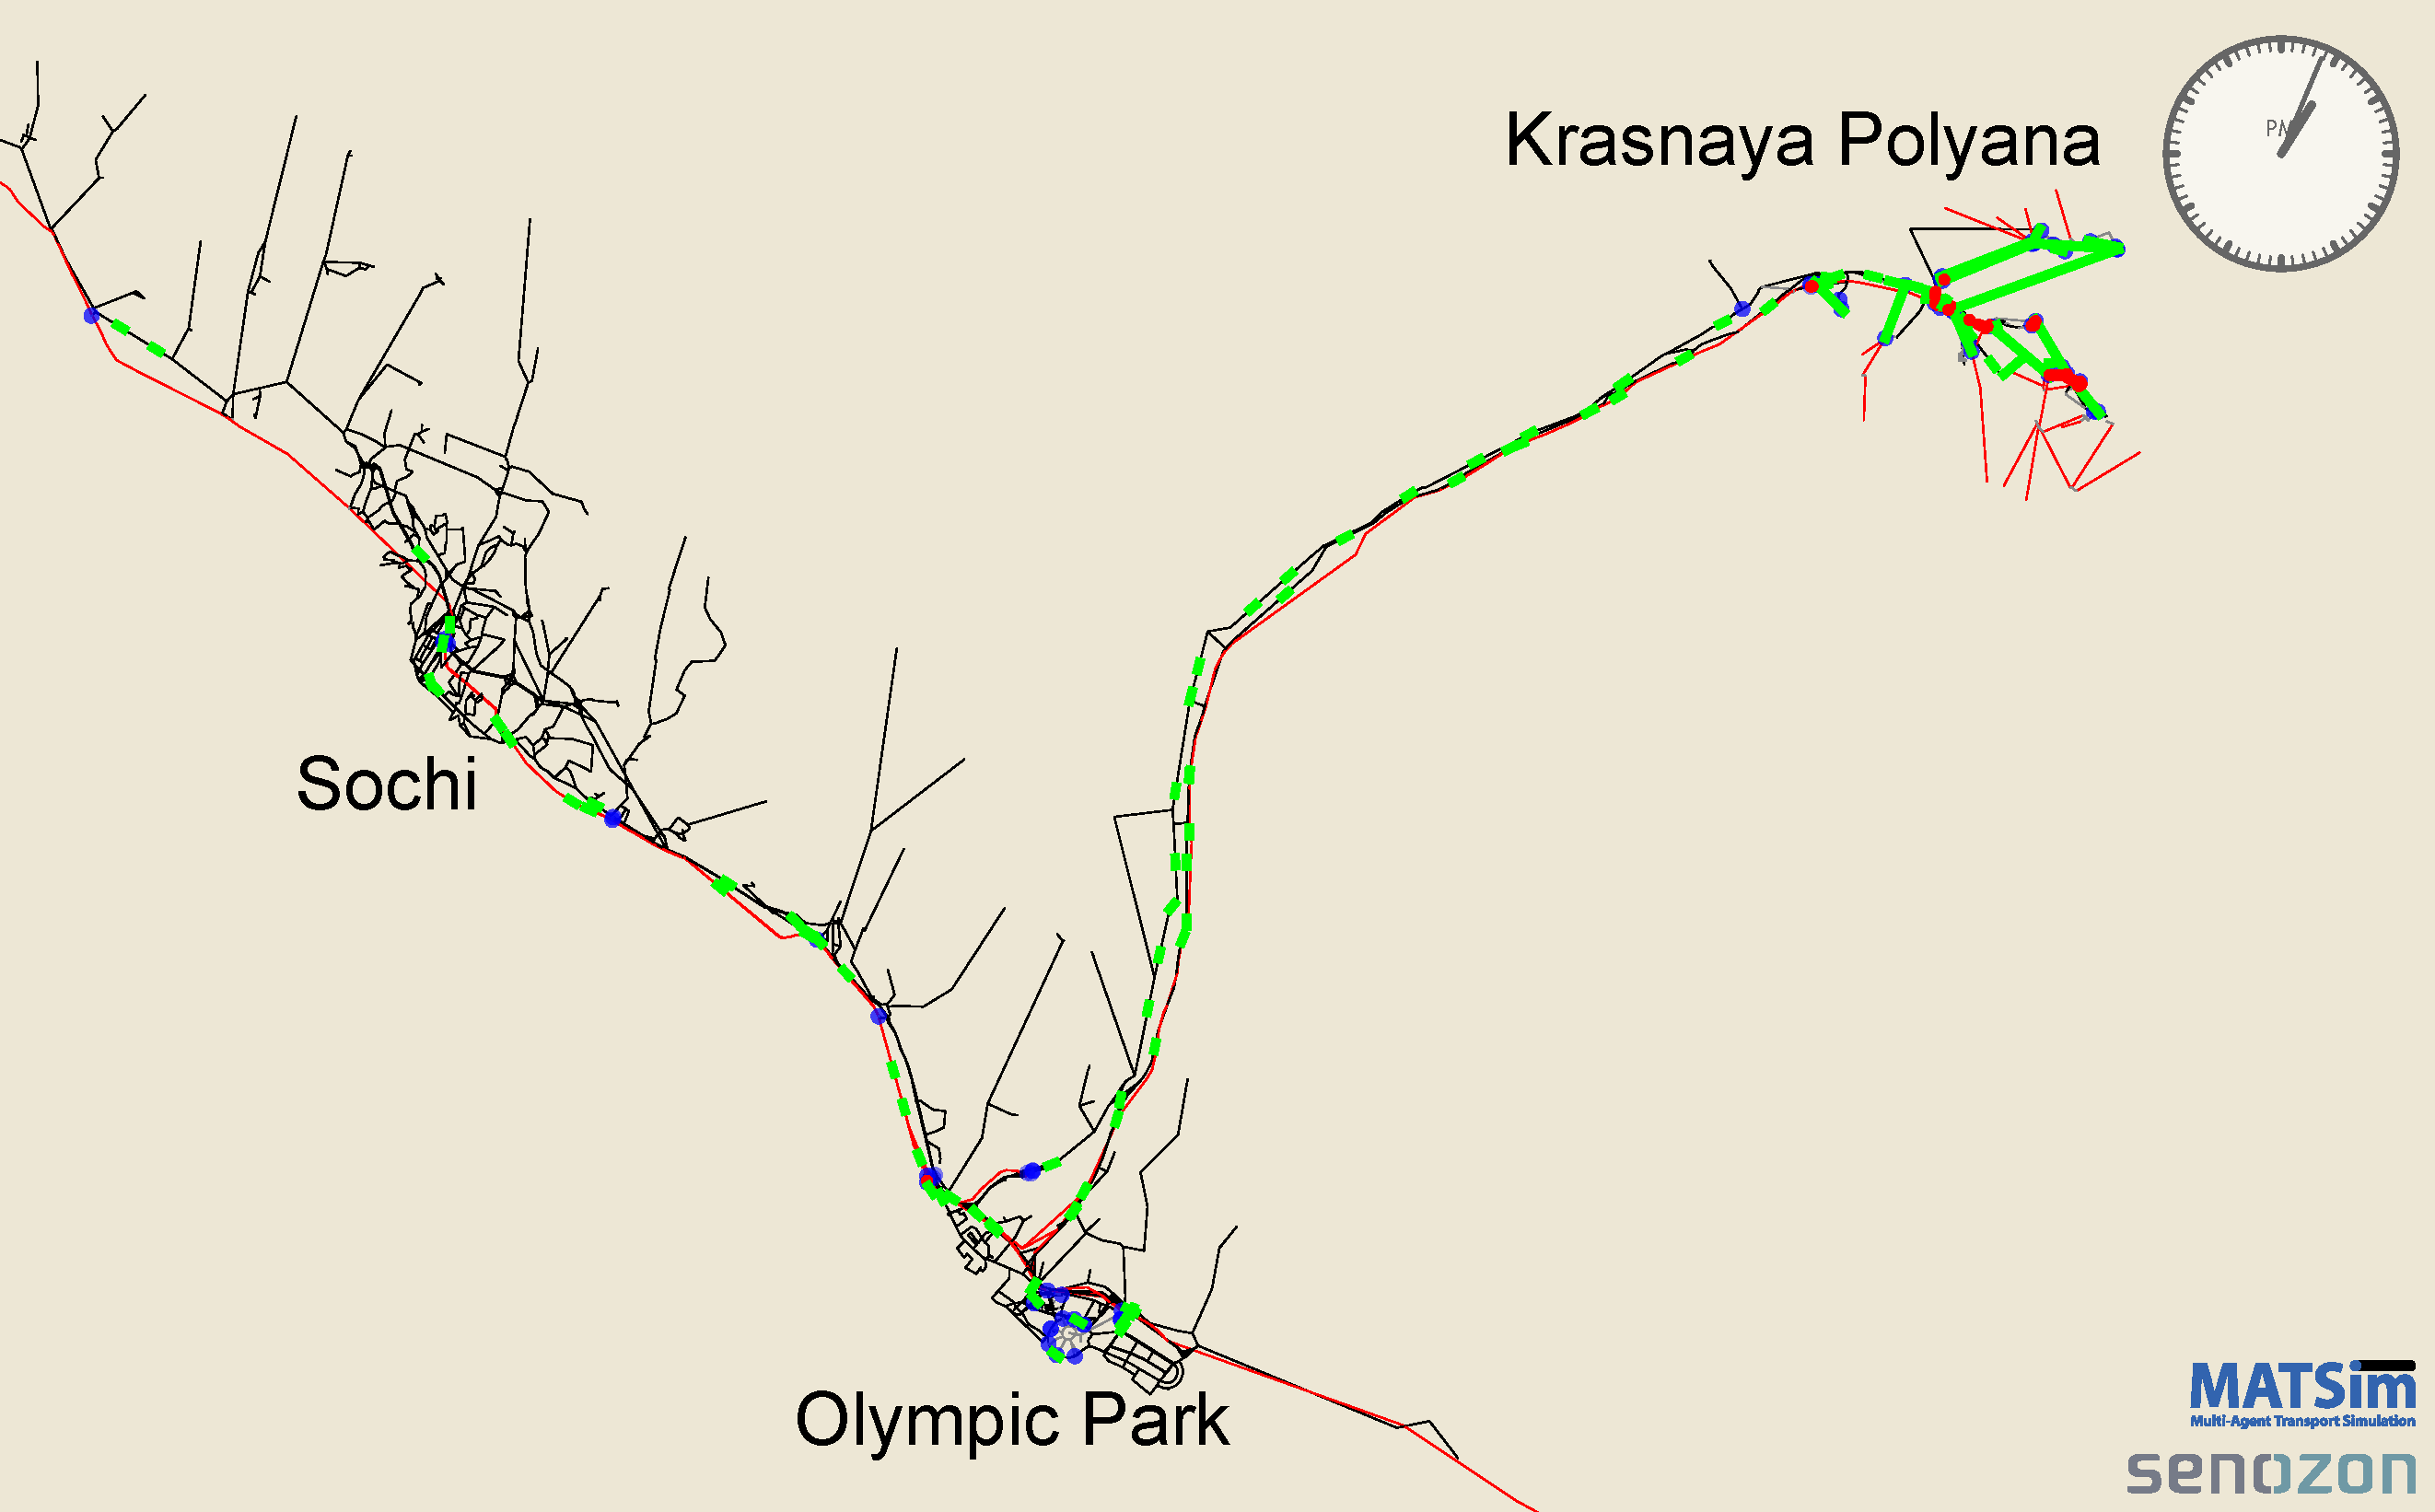
\includegraphics[width=1.\textwidth,angle=0]{./scenarios/figures/sochi_full.pdf}}%
{}
%

% ========================================================================================
\section{Outlook}
In addition to the test case of the 2014~Olympic winter games in Sochi, \gls{itsos}/\gls{matsim}
was also used to simulate traffic in St.\ Johann (Pongau, Austria), with particular 
emphasis on pupils, who often must take a combination of buses and trains to
get to school.

A new company, Masterconcept Mobility \gls{gmbh}, was split off from Masterconcept Consulting \gls{gmbh} in 2014; 
this new firm offers major event transportation planning services, as well as regional planning services 
based on the combination of \gls{itsos} and \gls{matsim}.

% ##################################################################################################################